\subsubsection{Top Yukawa-induced electroweak corrections}

\label{EW:Top-Higgs_sector}

%\paragraph{Authors:}
%\begin{itemize}
%    \item Margarete Mühlleitner, Johannes Schlenk, Michael Spira~\cite{Muhlleitner:2022ijf};
%    \item Arunima Bhattacharya, Francisco Campanario, Sauro Carlotti, Jamie Chang, Javier Mazzitelli, Margarete Mühlleitner, Jonathan Ronca, Michael Spira ~\cite{Bhattacharya_TBA}.
%\end{itemize}

\noindent \textbf{Milada Margarete Mühlleitner, Johannes Schlenk, Michael Spira~\cite{Muhlleitner:2022ijf}.}

\noindent The first calculation of partial electroweak corrections to Higgs boson pair production via the dominant gluon-fusion process has been performed by investigating the corrections induced by the top Yukawa coupling \cite{Muhlleitner:2022ijf}. In order to set up a complete and consistent framework, these corrections have been obtained in the gaugeless limit, where all electroweak gauge couplings are set to zero, but the (massless) Goldstone contributions are taken into account, see Fig.~\ref{fig:bd}. This approach ensures the preservation of the $SU(2)$ symmetry of the scalar Higgs doublet. While the top-induced corrections to the trilinear Higgs boson self-coupling vertex are treated with the full top quark mass dependence, the triangle and box diagrams involving couplings of one or two Higgs bosons to gluons are treated in the HTL. The corresponding diagrams are displayed in Fig.~\ref{fg:dia_htl}, where the first two represent those that are treated in the HTL. For these two diagrams, we have used the effective Lagrangian \cite{Djouadi:1994ge,Muhlleitner:2022ijf}
\begin{equation}
{\cal L}_{eff} = \frac{\alpha_s}{12\pi} G^{a\mu\nu} G^a_{\mu\nu} \left\{
(1+\delta_1) \frac{H}{v} + ( 1 + \eta_1) \frac{H^2}{2v^2} + {\cal
O}(H^3) \right\}
\label{eq:leff}
\end{equation}
where
\begin{eqnarray}
\delta_1 & = & \frac{x_t}{2} + {\cal O}(x_t^2) \,, \qquad\qquad
\eta_1   = 4 x_t + {\cal O}(x_t^2) \,,
\label{eq:leff_coeff}
\end{eqnarray}
Here $x_t = G_F m_t^2/(8\sqrt{2}\pi^2)$, $G_F$ denotes the Fermi constant, $v$ is the vacuum expectation value (vev) of the Higgs field, and $m_t$ is the top quark mass. This effective Lagrangian describes the electroweak corrections induced by $x_t$ to the $hgg$ and $hhgg$ vertices in the HTL. We would like to point out explicitly that the square root of the wave-function counterterm of the external Higgs boson(s) is already taken into account in this effective Lagrangian.
\begin{figure}[!hbtp]
\centering
%\vspace*{-1.6cm}
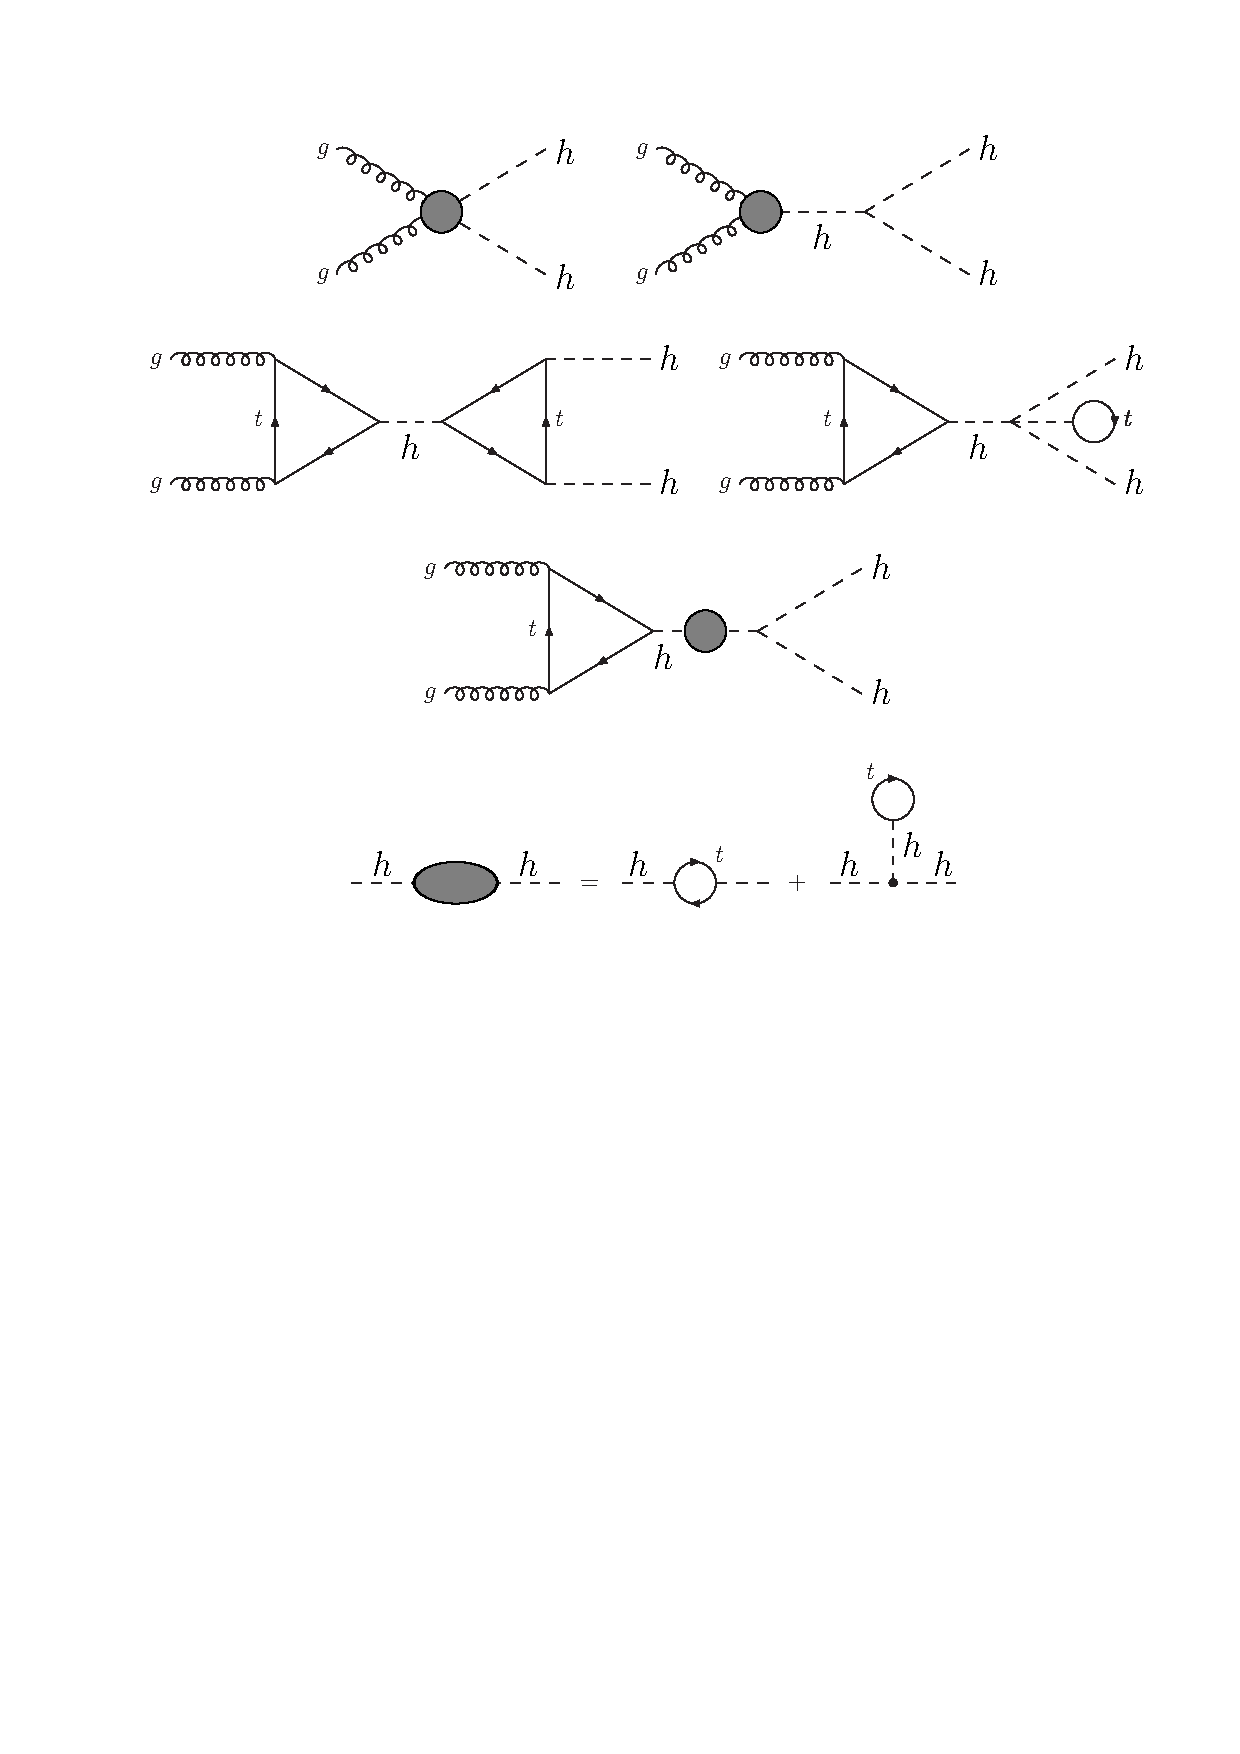
\includegraphics[width=0.9\textwidth]{NLO_EW_SM/EW_top-Higgs_sector/Images/dia_htl_hlabels.pdf}
%\vspace*{-8.3cm}
\caption{\label{fg:dia_htl}Generic diagrams contributing to the top Yukawa-induced electroweak corrections to the $gg\to hh$ process. The first two diagrams have been treated in the HTL. Diagrams adapted from Ref.~\cite{Muhlleitner:2022ijf}.}
\end{figure}
In Fig.~\ref{fg:dia_htl} the tadpole diagrams are displayed explicitly. We have used both the Fleischer--Jegerlehner scheme and the conventional scheme, in which the tadpole diagrams are omitted but retained in the corresponding counterterm of the trilinear Higgs boson self-coupling. We have obtained identical results in the final sum of the radiative corrections, once the vev $v$ is expressed in terms of the Fermi constant $G_F$.

Because the full top quark mass dependence of the one-loop times one-loop diagrams describing the radiatively corrected trilinear Higgs boson self-coupling vertex (all diagrams of Fig.~\ref{fg:dia_htl} except the first two) has been kept, the use of the effective trilinear Higgs boson self-coupling (derived from the effective Coleman--Weinberg potential \cite{Coleman:1973jx,Weinberg:1973ua,Jackiw:1974cv})
\begin{equation}
\lambda_{hhh} = 3 \frac{m_h^2}{v} \, , \qquad\qquad \lambda_{hhh}^{\rm eff} = \lambda_{hhh} - \frac{3 m_t^4}{\pi^2 v^3} \approx 0.91 \times \lambda_{hhh}
\end{equation}
to accommodate the dominant part of the radiative corrections can be tested. The result is that process-dependent, finite-momentum-dependent corrections are of the same size as the corrections above, growing with $m_t^4$,
\begin{eqnarray}
\sigma & = & K_{elw} \times \sigma_{LO} \nonumber \\
K_{elw} & \approx & 1.002 \hspace*{1.0cm} \mbox{($\lambda_{hhh}$)} \nonumber \\
K^{eff}_{elw} & \approx & 0.938 \hspace*{1cm} \mbox{($\lambda^{\rm eff}_{hhh}$)}.
\end{eqnarray}
Since the effective trilinear Higgs boson self-coupling generates about $6\%$ electroweak corrections to the total cross section artificially and larger corrections to the distributions, using the LO-like trilinear Higgs boson self-coupling $\lambda_{hhh}$ is favoured \cite{Muhlleitner:2022ijf}. The top Yukawa-induced electroweak corrections are small except in the region close to the production threshold due to the complete cancellation of the leading top quark mass terms in the LO matrix element, to which the corrections are normalized.

~

\noindent \textbf{Arunima Bhattacharya, Francisco Campanario, Sauro Carlotti, Jamie Chang, Javier Mazzitelli, Milada Margarete Mühlleitner, Jonathan Ronca, Michael Spira ~\cite{Bhattacharya_TBA}.}

\noindent The analysis of the top Yukawa-induced electroweak corrections discussed above has been extended to include the full top quark mass dependence. Specifically, the first two diagrams of Fig.~\ref{fg:dia_htl}, previously evaluated in the HTL, have been resolved into the corresponding two-loop diagrams involving top, bottom, Higgs, and Goldstone propagators. To preserve the SU(2) symmetry of the Higgs sector, this work has been performed in the gaugeless limit, enabling a gauge-invariant definition of the contributions associated with the top Yukawa coupling. In this limit, the Goldstone bosons are massless but do not generate infrared singularities. The method used for this calculation involves applying the projectors to the two form factors (in $D=4-2\epsilon$ dimensions), followed by a diagram-by-diagram Feynman parametrization. Since no tensor reduction has been used, the resulting Feynman integrands remain quite compact. The singularities were extracted by appropriate end-point subtractions. Moreover, this allowed us to keep, alongside the top quark mass, the bottom and the Higgs masses as free symbolic parameters. The virtual thresholds have been treated by introducing complex masses of the virtual propagators,
\begin{equation}
m_{t/b}^2 \to m_{t/b}^2 (1-i\bar\epsilon) \, , \qquad m_h^2 \to m_h^2 (1-i\bar\epsilon)
\end{equation}
with the regulator $\bar\epsilon$ to be sent to 0. The latter was achieved by applying a Richardson extrapolation \cite{Richardson} to a series of different values of $\bar\epsilon$. The minimal value of $\bar\epsilon$ used for numerical integrations varied between $10^{-8}$ and 0.1 depending on the diagram and the value of the invariant Higgs boson pair mass $Q=m_{hh}$. The top quark mass has been renormalized on-shell, and the vev has been renormalized according to the proper definition of the Fermi constant in muon decay.
\begin{figure}[!hbtp]
    \centering
    %\vspace*{-1.5cm}
    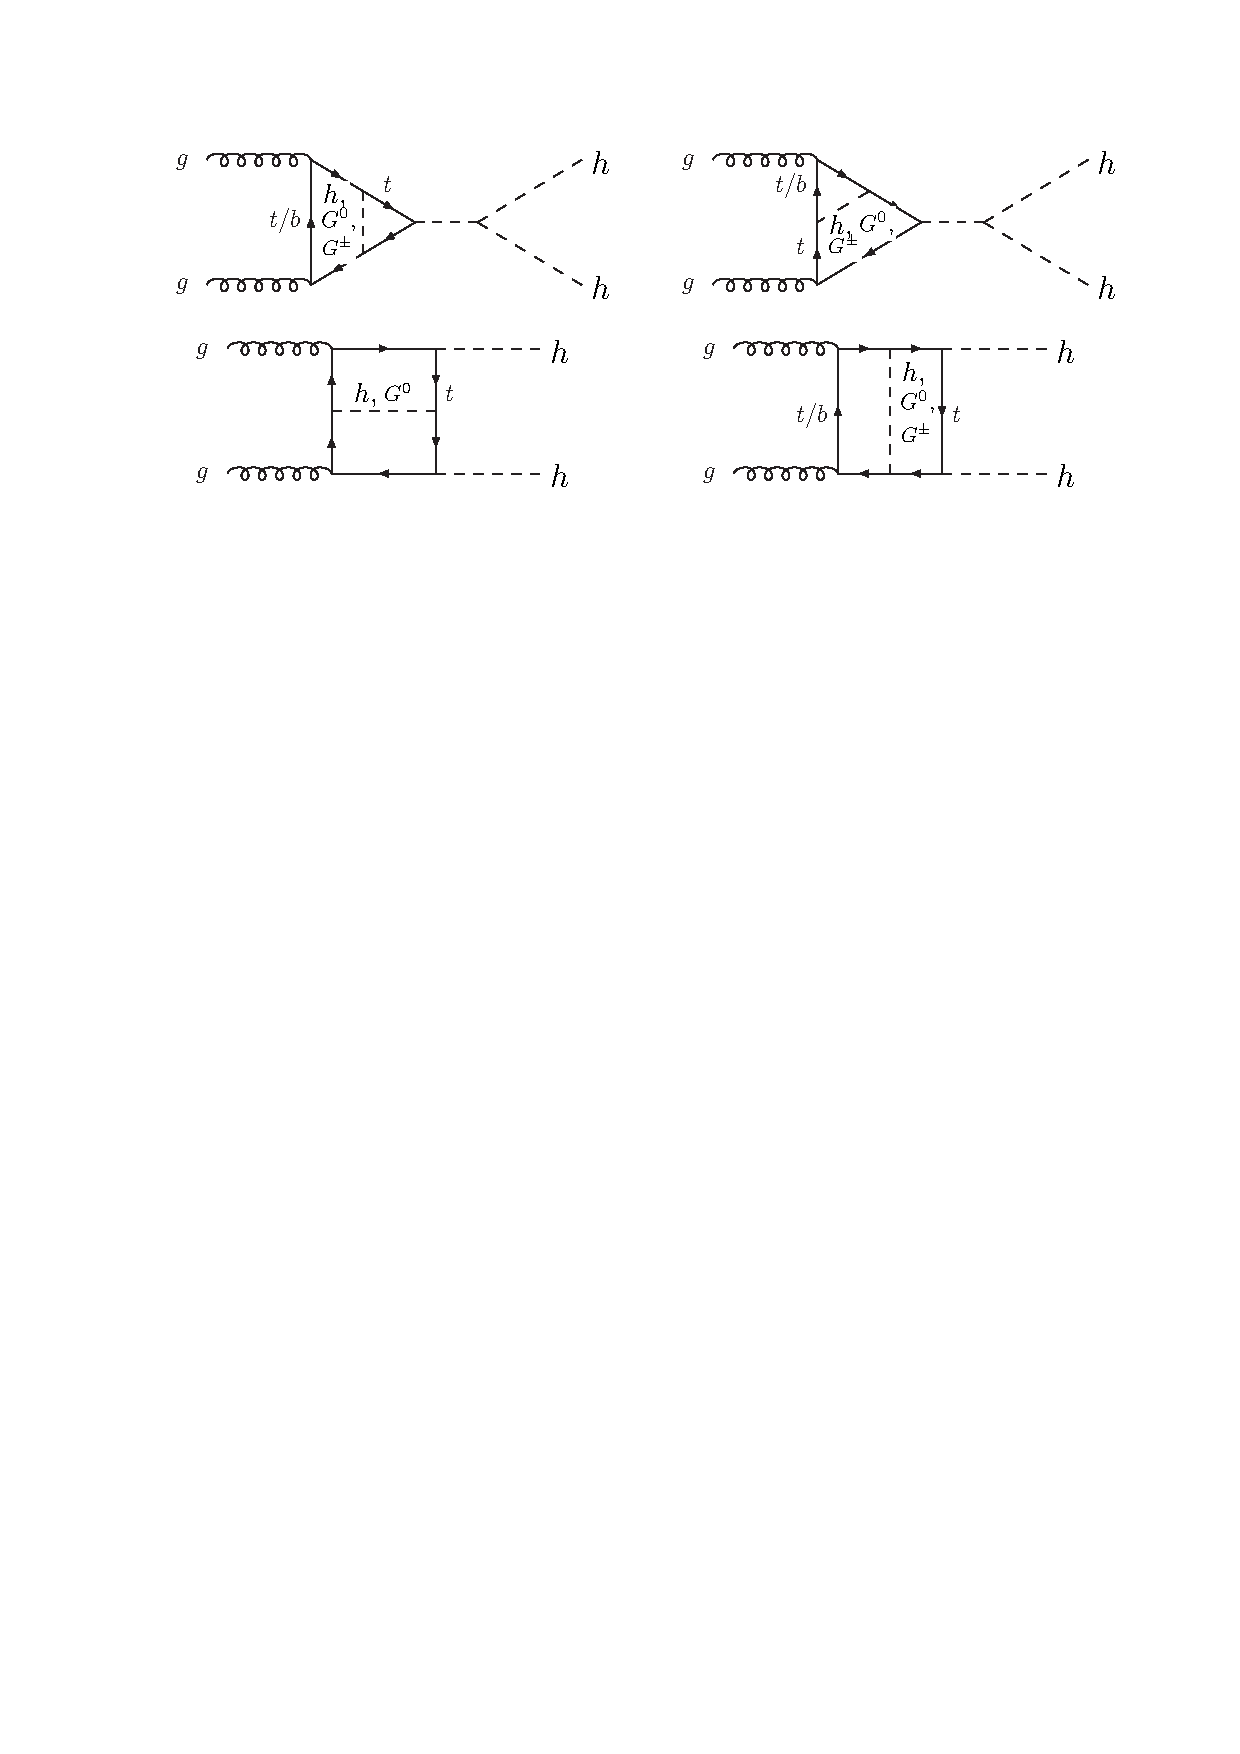
\includegraphics[width=0.8\textwidth]{NLO_EW_SM/EW_top-Higgs_sector/Images/dia_top_hlabels.pdf}
    %\vspace*{-13.9cm}
    \caption{\label{fg:dia_top}Sample two-loop triangle and box diagrams of the top Yukawa-induced electroweak corrections to Higgs boson pair production involving Higgs $h$ and Goldstone $G^0,G^\pm$ exchanges. The bottom propagators only contribute to the diagrams with charged Goldstone exchange. Diagrams from Ref.~\cite{Bhattacharya_TBA}.}
\end{figure}
\begin{figure}[!hbtp]
    \centering
    %\vspace*{-7cm}
    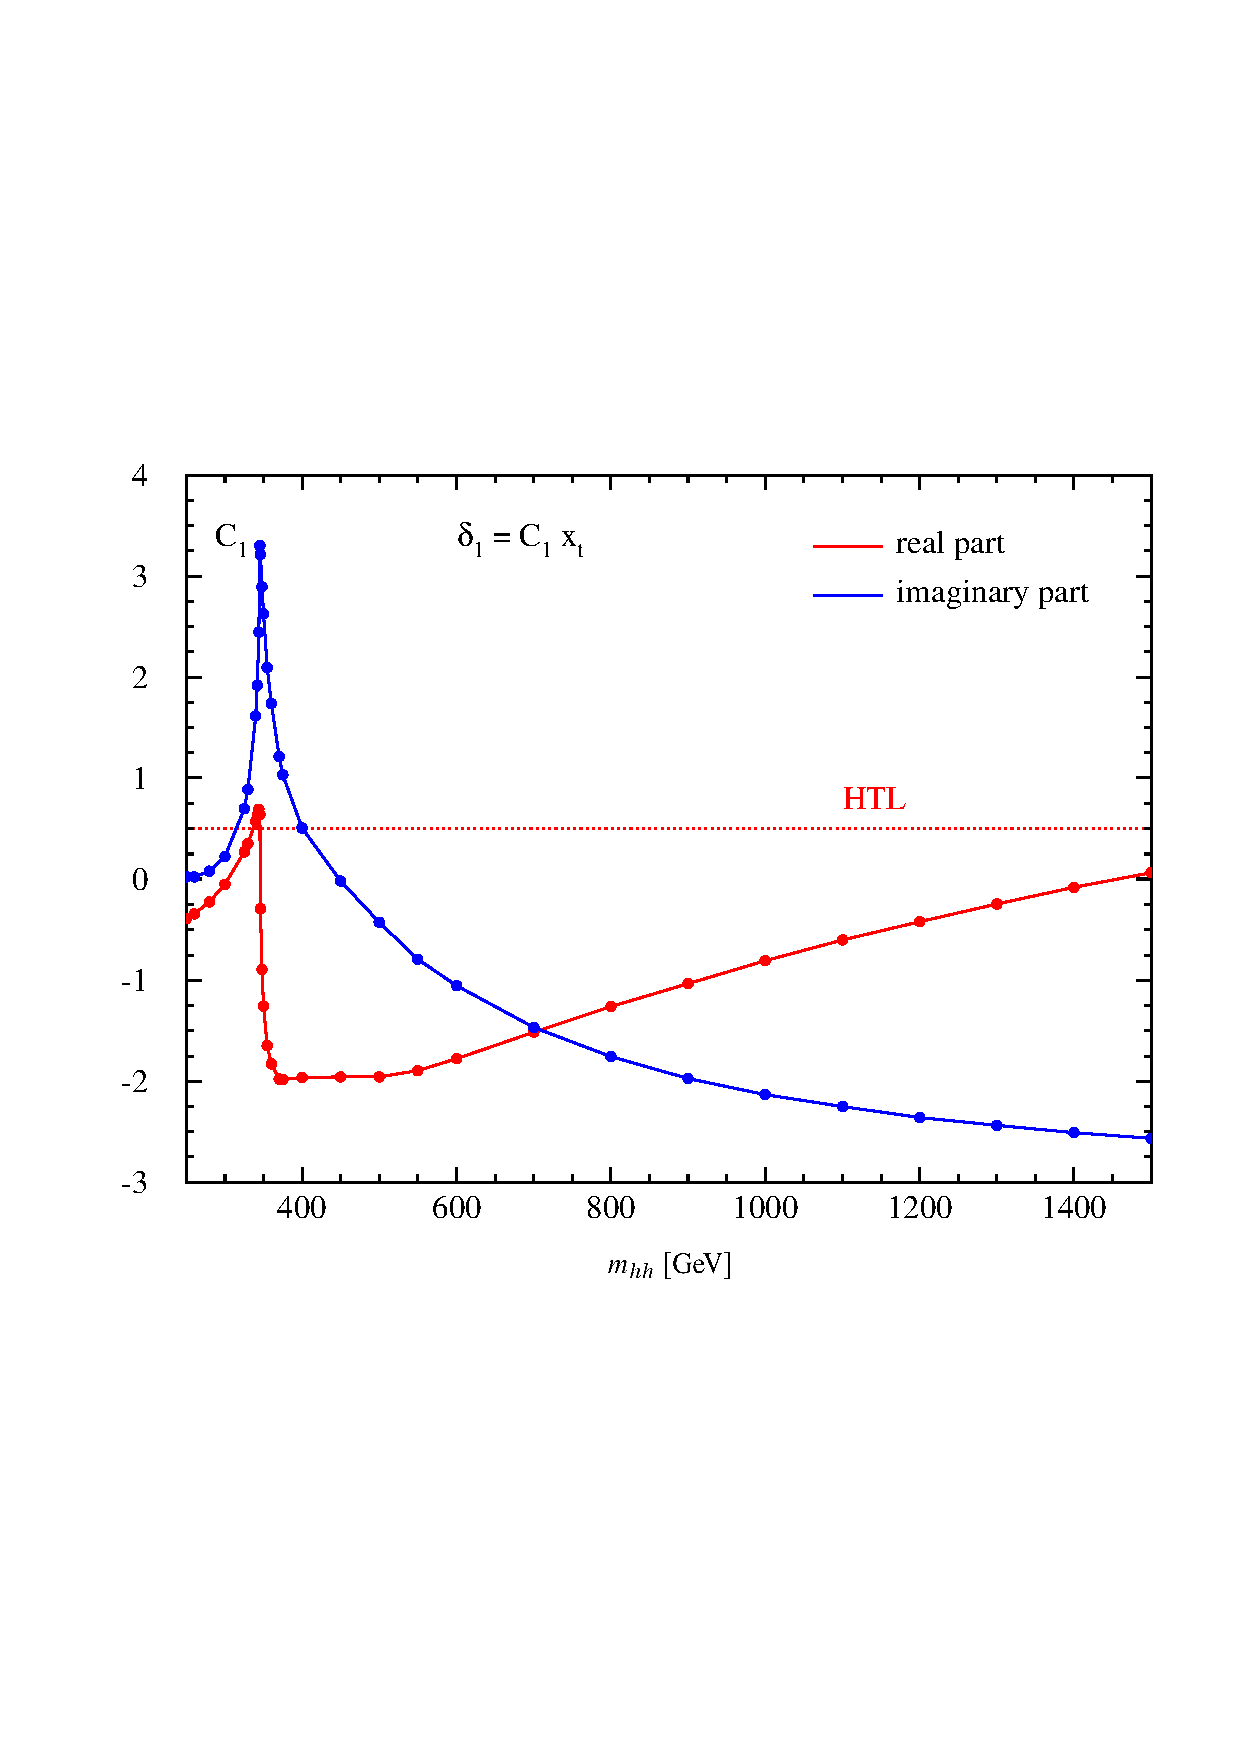
\includegraphics[width=0.7\textwidth]{NLO_EW_SM/EW_top-Higgs_sector/Images/d1tria_mhh.pdf}
    %\vspace*{-4.7cm}
    \caption{\label{fg:delta_1}The full top quark mass dependence of the coefficient $\delta_1$ of Eq.~\eqref{eq:leff_coeff} as a function of the invariant Higgs boson pair mass. The dotted line shows the purely real HTL result. The sizeable imaginary part arises from the diagrams with charged Goldstone exchange that include diagrams with $b\bar b$ thresholds. The points on the curve indicate the $m_{hh}$ values for which $\delta_1$ has been computed. The numerical errors are negligible and thus not shown. Results shown are from Ref.~\cite{Bhattacharya_TBA}.}
\end{figure}

The result of the two-loop triangle diagrams, see Fig.~\ref{fg:dia_top}, which can be directly compared to the coefficient $\delta_1$ in Eq.~\eqref{eq:leff_coeff}, is shown in Fig.~\ref{fg:delta_1}. As a cross-check, the HTL result of Eq.~\eqref{eq:leff_coeff} has been reproduced within uncertainties by artificially increasing the value of the top quark mass. The results indicate differences between the HTL and the full result at the (sub)percent level for the distribution in the Higgs boson pair mass.

The calculation of the two-loop box diagrams, see Fig.~\ref{fg:dia_top}, is more involved, since the additional phase space dependence does not allow for an immediate comparison with the HTL. Applying the same method as for the two-loop triangle diagrams and including the phase space integration in the numerical analysis, the result of the two-loop renormalized box diagrams plus the two-loop triangle diagrams and the previous one-loop times one-loop diagrams related to the radiative corrections to the trilinear Higgs boson self-coupling vertex is shown in Fig.~\ref{fg:del_top}, where the relative corrections are defined as
\begin{equation}
\sigma (gg\to hh) = \sigma_{LO} (gg\to hh)~( 1 + \delta_{\text{top Yukawa}} + \delta_{\text{light quarks}} )
\end{equation}
with the light-quark contributions $\delta_{\text{light quarks}}$ discussed in Section~\ref{EW:light-quark}. The total corrections are about $-5\%$ for intermediate values of $m_{hh}$ and are smaller for large values, while they are large close to the production threshold due to the large cancellation in the LO matrix element, to which the corrections are normalized. At large values of $m_{hh}$, the corrections develop a visible slope. The right panel of Fig.~\ref{fg:del_top} shows details of the $t\bar t$ threshold, which develops a sign-changing interference behaviour with the LO matrix element, with a maximum below the $t\bar t$ threshold.
\begin{figure}[!hbtp]
    \centering
    %\vspace*{-3.5cm}
%    \subfloat[]{{
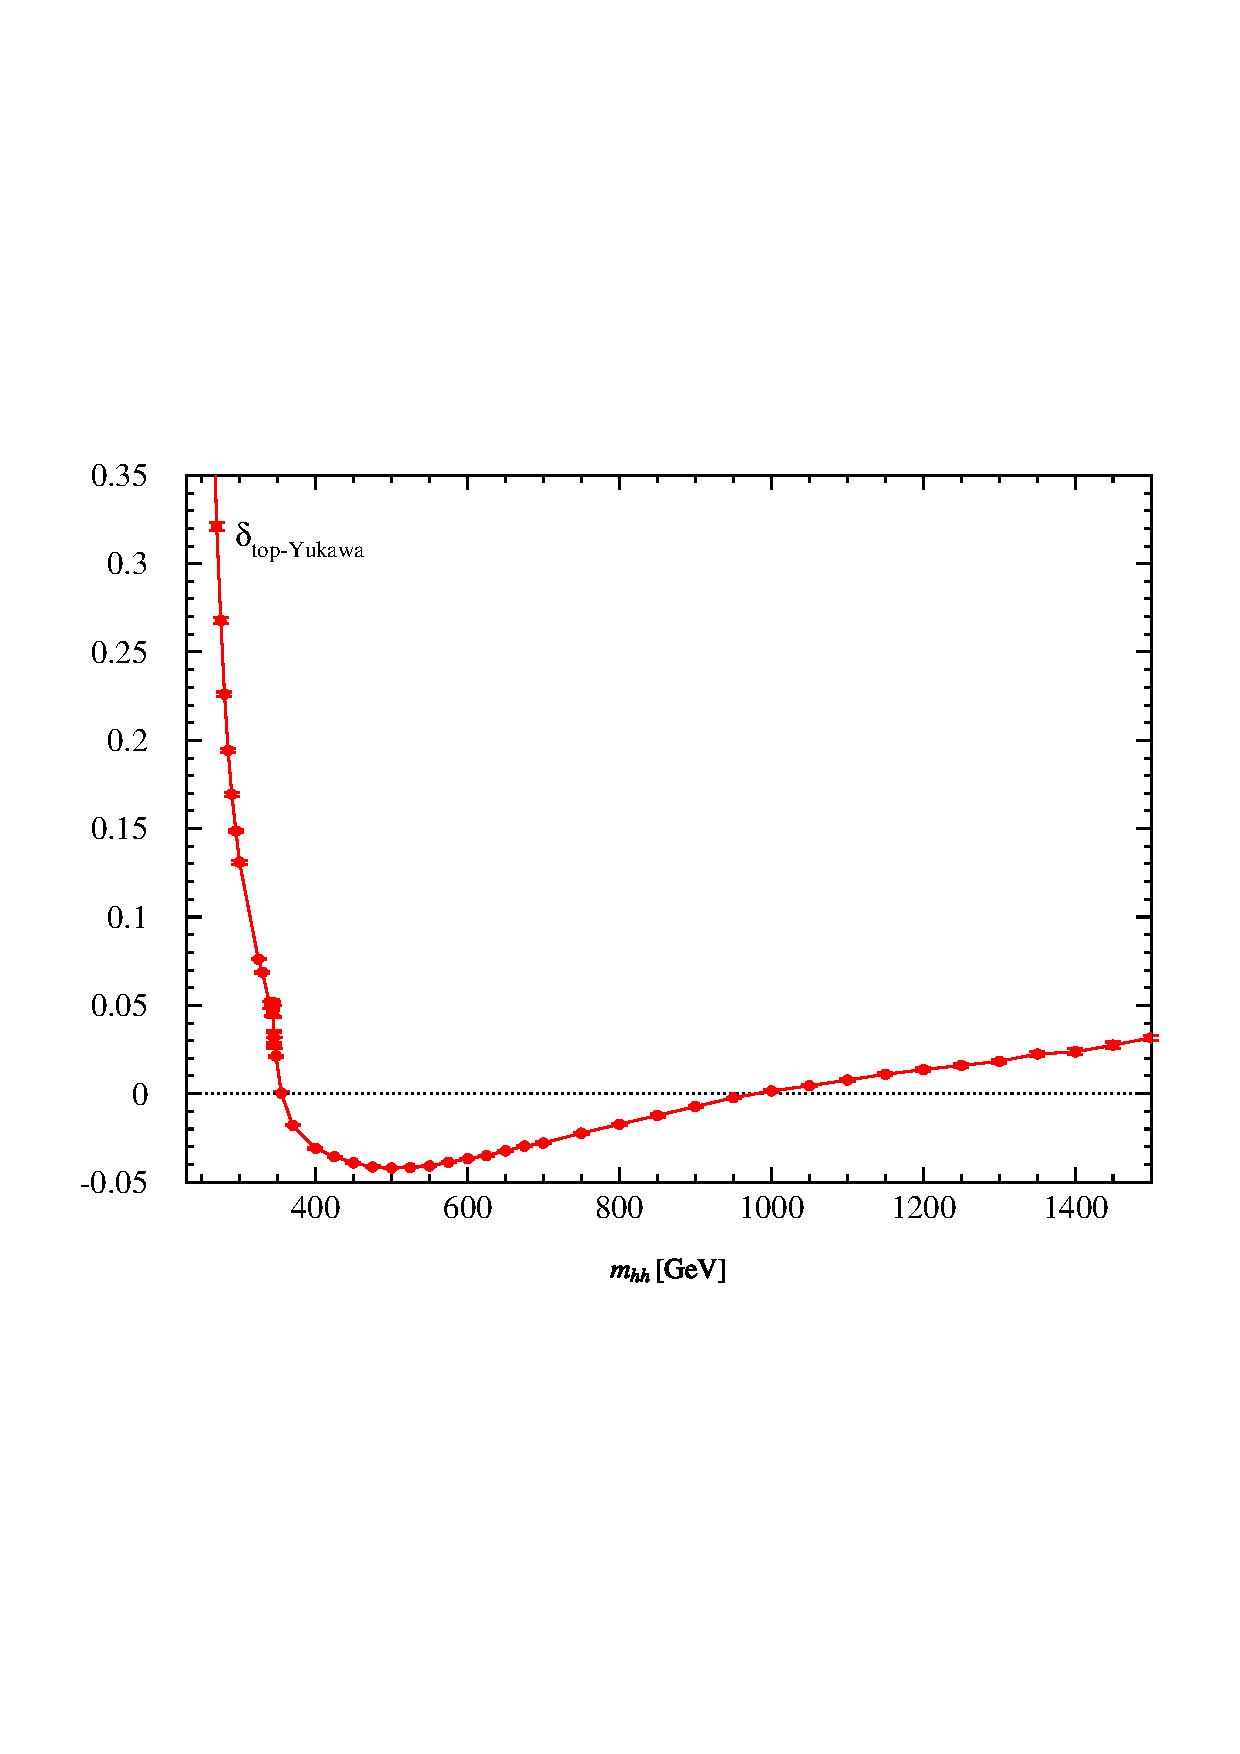
\includegraphics[width=0.49\textwidth]{NLO_EW_SM/EW_top-Higgs_sector/Images/del_top_mhh.pdf}
%}}
    %\vspace*{-10cm}
    %\%hspace*{-1.0cm}
%    \subfloat[]{{
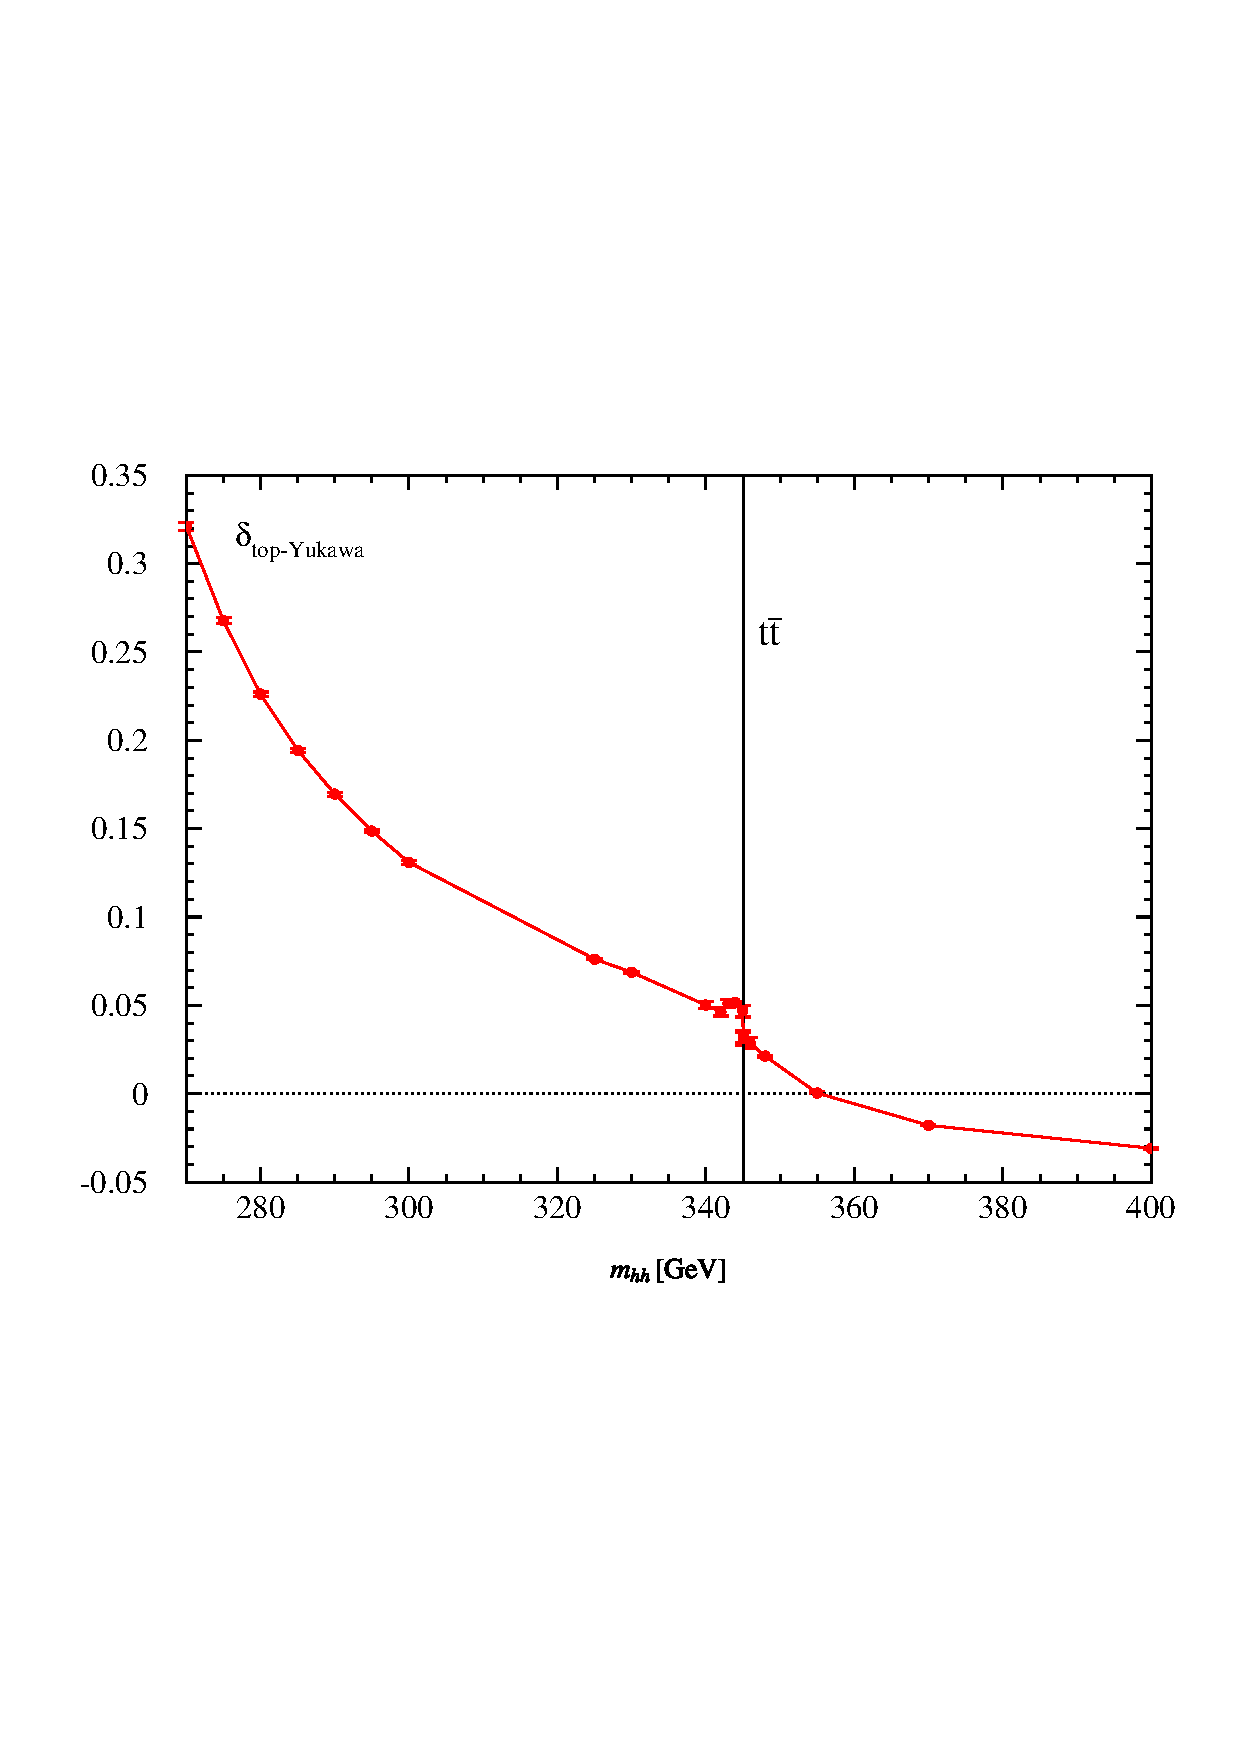
\includegraphics[width=0.49\textwidth]{NLO_EW_SM/EW_top-Higgs_sector/Images/del_top.detail_mhh.pdf}
%}}
    %\vspace*{6.0cm}
    \caption{The full relative top Yukawa-induced electroweak corrections to the $gg \to hh$ process. The points on the curve indicate the $m_{hh}$ values for which the corrections have been computed. The right panel shows a magnified view of the structure of the $t\bar t$ threshold. Numerical error bars are shown for each point. The vertical line indicates the position of the $t\bar t$ threshold. Results shown are from Ref.~\cite{Bhattacharya_TBA}.}
    \label{fg:del_top}
\end{figure}
